%%%%%%
%
% $Autor: Srikanth Nanda $
% $Datum: 2025-09-27 11:15:45Z $
% $Pfad: githubtemplate/Template/Presentations/Template/slides/rename.tex $
% $Version: 4620 $
%
%
% !TeX encoding = utf8
% !TeX root = Rename
%
%%%%%%


\Mysection{Introduction to Floor Localization}

\STANDARD{Introduction}
{
	Image-based floor detection also known as Floor Localization is a key task in mobile robot navigation. It provides the robot with information about the free space in its environment, allowing safe movement and obstacle avoidance. Detecting the floor also supplies structural cues, such as the boundary between floor and walls, which are useful for generating maps of indoor spaces.\cite{Li:2010}

	\pagebreak
	\begin{figure}
		\centering 
		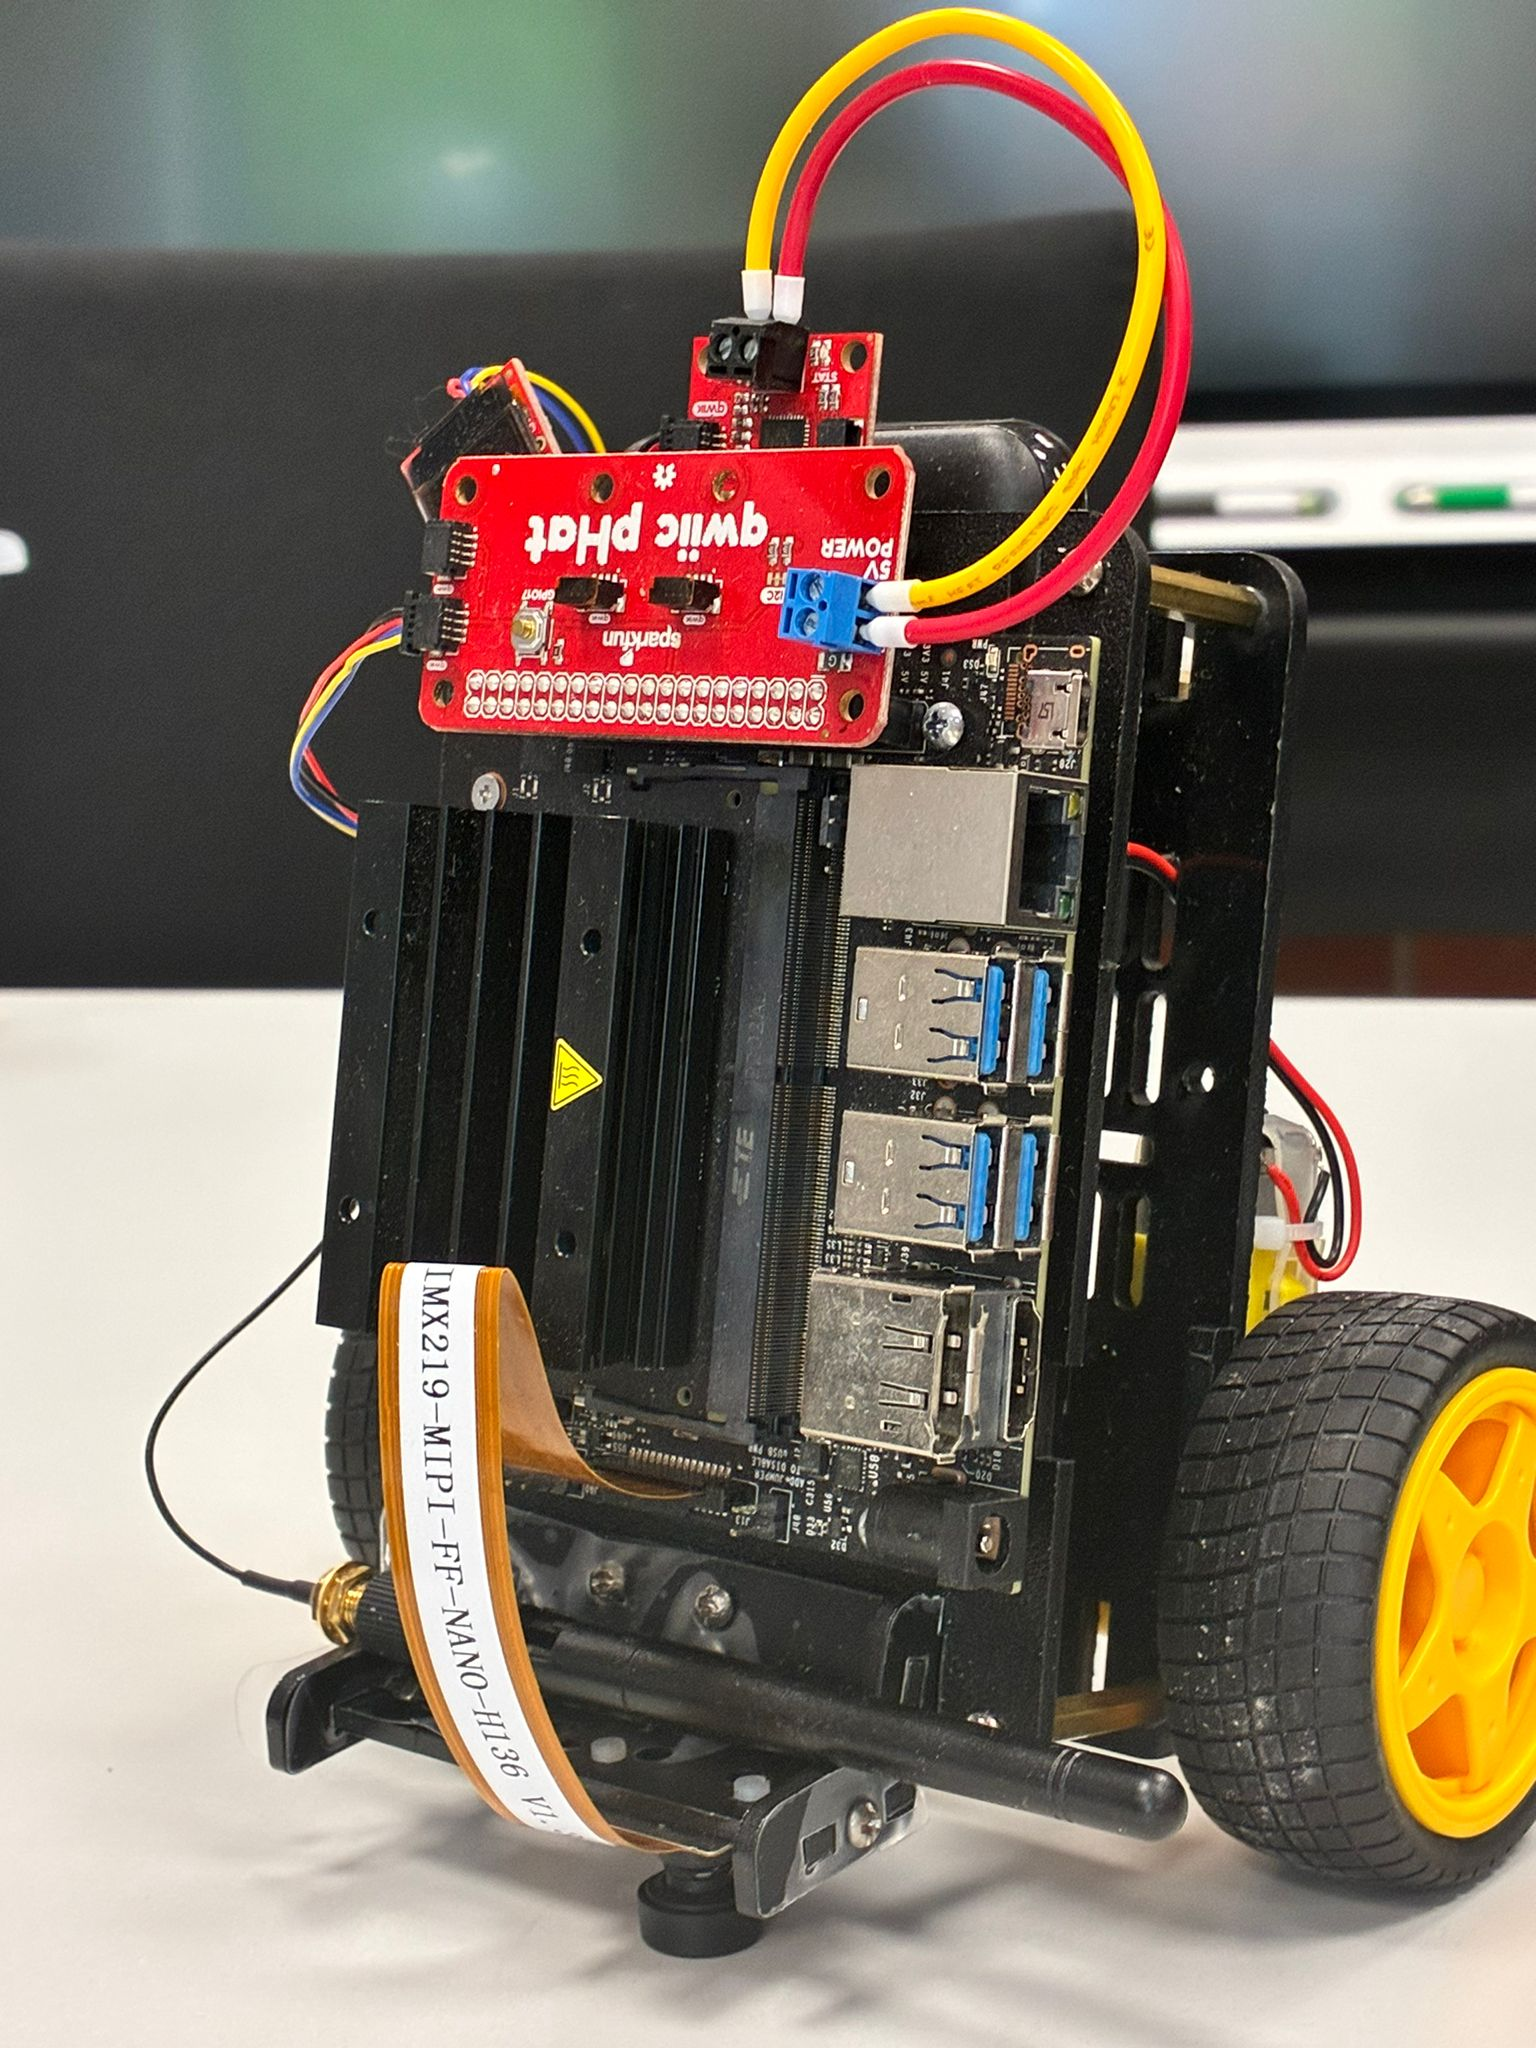
\includegraphics[width=0.4\linewidth]{../FloorLocalization/images/robot1.jpeg}
		\caption{Mobile Robot Implemented using Nvidia Jetson Nano(Top view)}
	\end{figure}
	\pagebreak
	\begin{figure}
		\centering 
		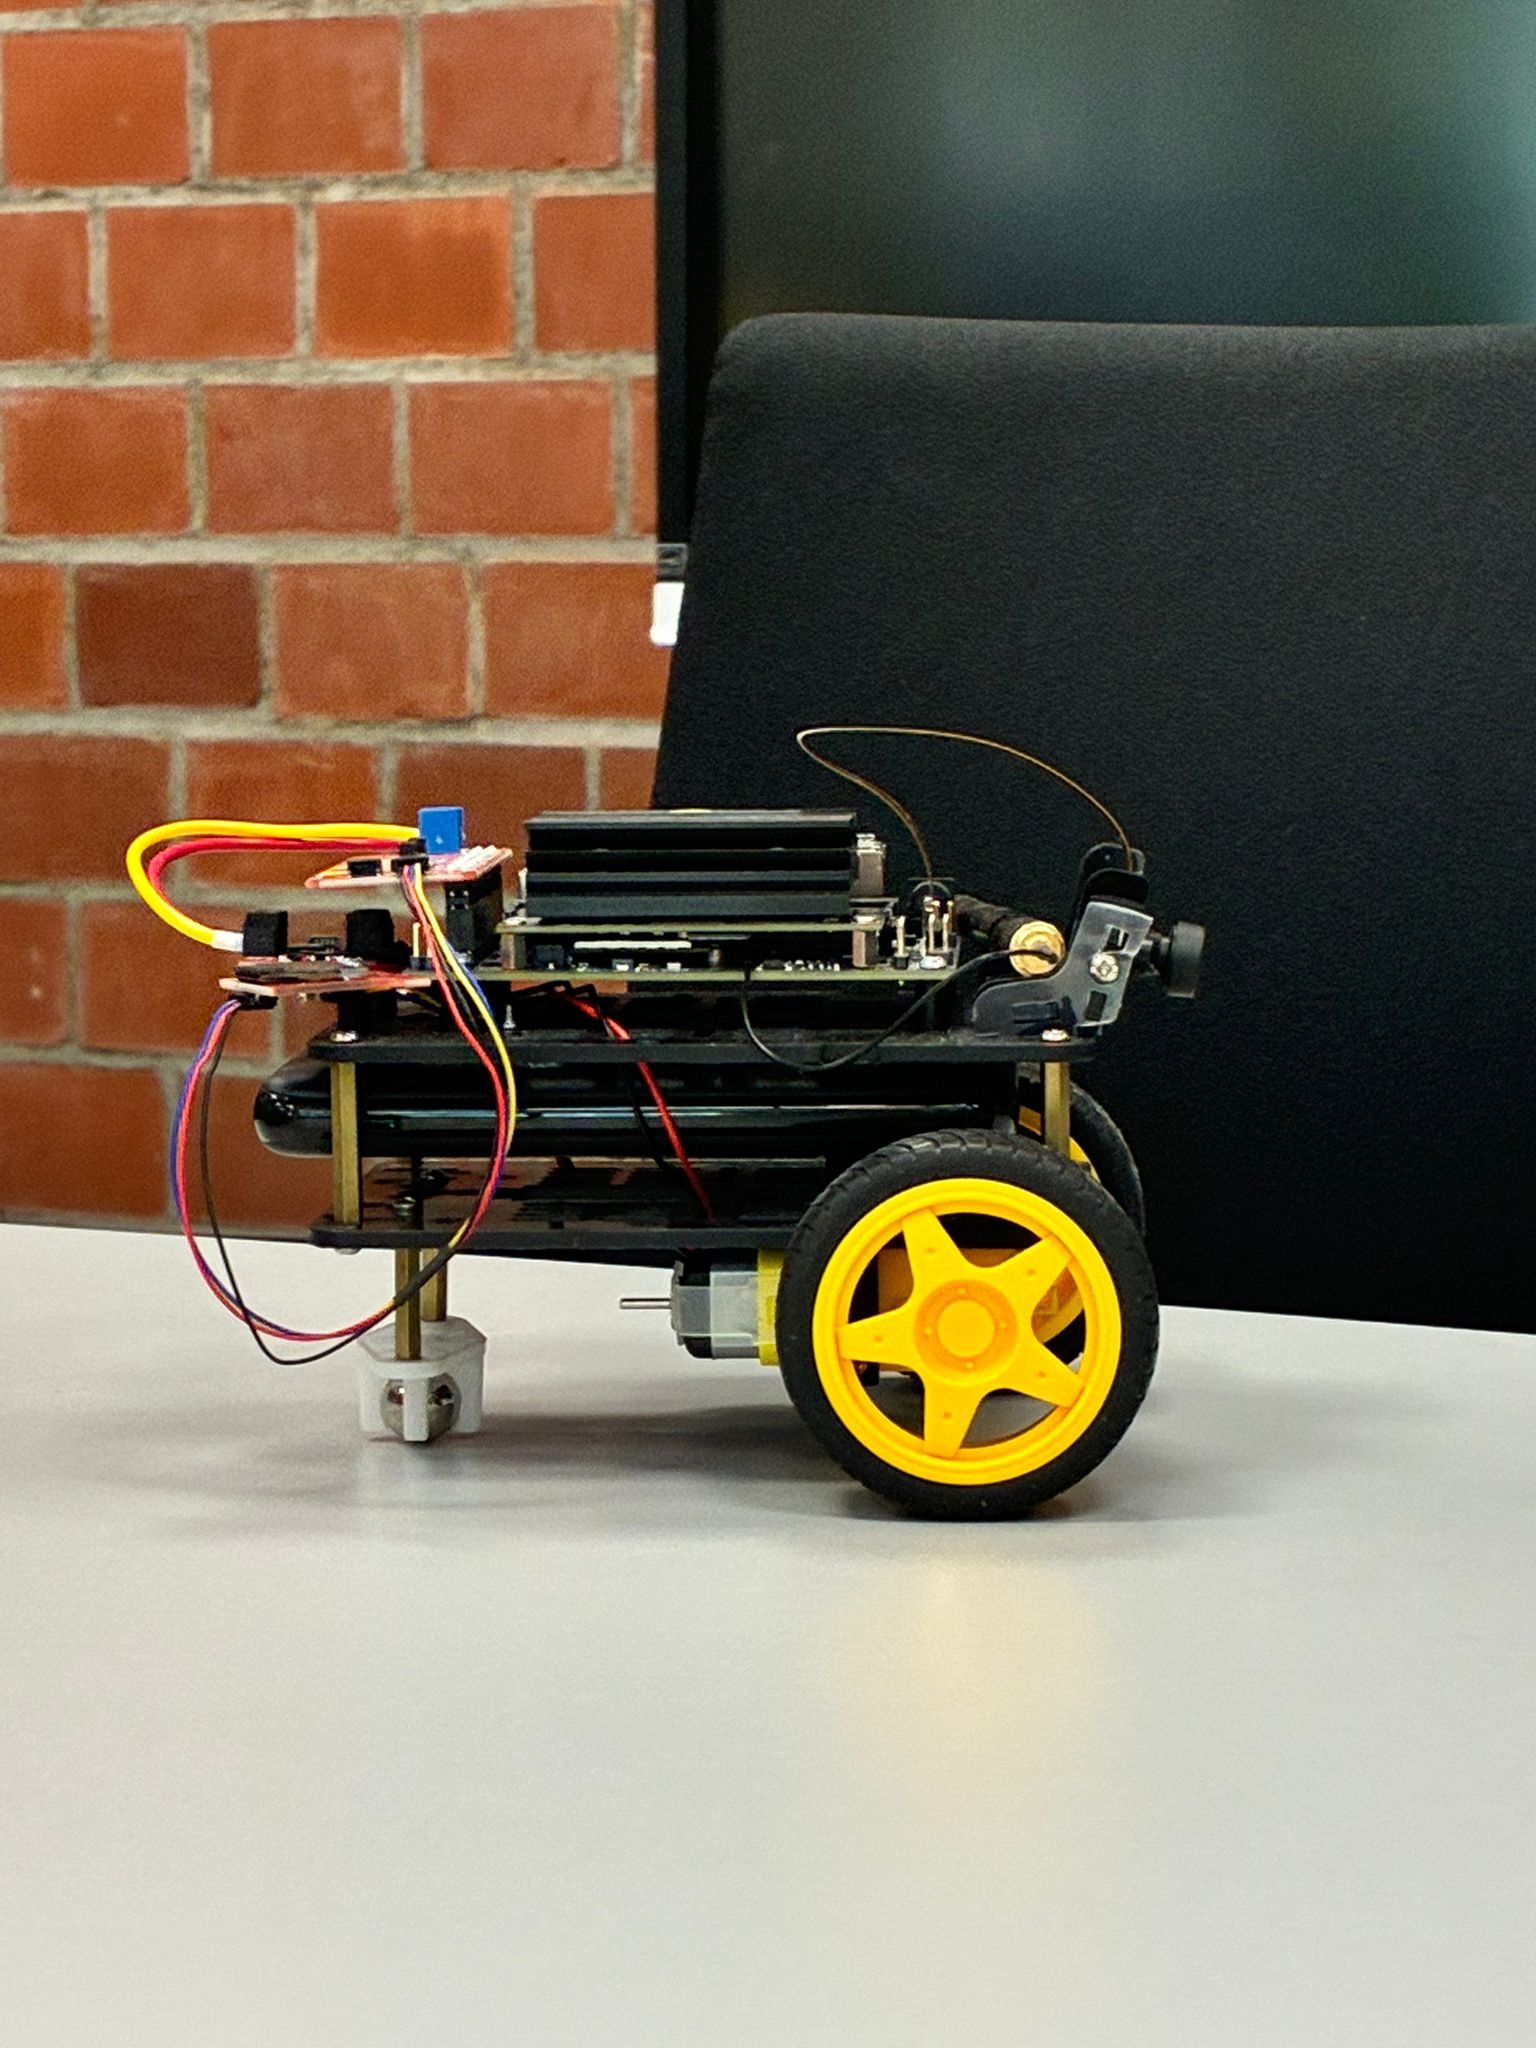
\includegraphics[width=0.4\linewidth]{../FloorLocalization/images/RobotImplemented.jpeg}
		\caption{Mobile Robot Implemented using Nvidia Jetson Nano(Side view)}
	\end{figure}
	
}
{
\STANDARD{During Localization}
{
	During localization, the identified floor region can be matched with the floor layout in an existing map to support accurate position estimation. Floor detection further enables the calculation of spatial metrics, including the usable area or the dimensions of a room. In this work, these functions are implemented on a four-wheel rover using an NVIDIA Jetson Nano and a Raspberry Pi 2-megapixel camera, building on earlier work in vision-based floor segmentation.\cite{Li:2010}
}
\STANDARD{Ground Texture Localization}
{
	\begin{figure}
		\centering 
		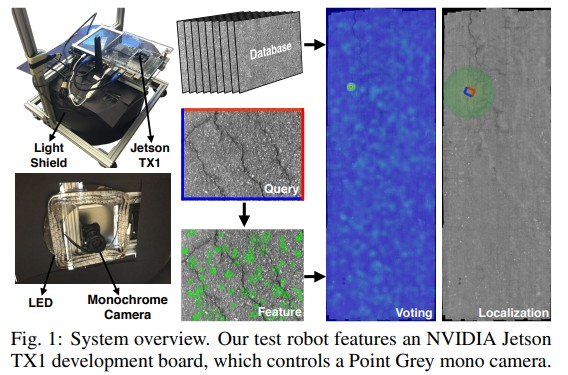
\includegraphics[width=0.75\linewidth]{../FloorLocalization/images/groundtexturelocalization.jpg}
		\caption{Extracting Ground Texture \cite{Zhang:2019}}
	\end{figure}
	
}

\Mysection{Challenges, Solution and Applications}
\STANDARD{Challenges}
{
   \textbf{Indoor Navigation Challenges}

   Indoor positioning systems face several fundamental challenges that make them significantly more complex than their outdoor counterparts:

   \begin{itemize}
        \item \textbf{GPS Signal Unavailability}: Global Navigation Satellite Systems (GNSS) signals are severely attenuated or completely blocked in indoor environments, subterranean locations, and dense urban environments \cite{Pasricha:2024}.  
		\item \textbf{Signal Propagation Issues}: Indoor wireless signals suffer from multipath fading, shadowing effects, and reflection interference from walls, furniture, and other obstacles \cite{Affan:2023}.	
		\pagebreak
		\begin{figure}
			\centering 
			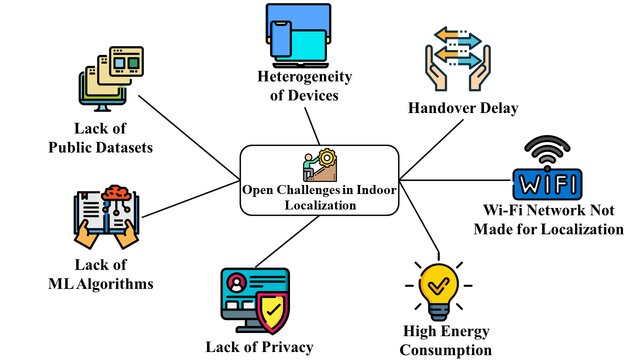
\includegraphics[width=0.75\linewidth]{../FloorLocalization/images/Challenges.jpg}
			\caption{Indoor Navigation Challenges \cite{Caltagirone:2021}}
		\end{figure}
		\pagebreak	       
		\item \textbf{Dynamic Environment Complexity}: Indoor spaces contain moving objects, varying lighting conditions, and changing layouts that challenge traditional localization algorithms \cite{Linus:2023}.			       
		\item \textbf{Computational Constraints}: Mobile and embedded systems have limited processing power, memory, and energy resources for complex localization algorithms \cite{Tiku:2021}.
	\end{itemize}
}

\STANDARD{Solutions}
{
	Computer vision offers robust solutions for indoor localization through several key approaches:

	\begin{itemize}
	    \item \textbf{Visual Simultaneous Localization and Mapping (VSLAM)}: Constructs environmental maps while tracking camera pose using feature extraction and matching algorithms \cite{Bamdad:2024}.  
		\item \textbf{Deep Learning Integration}: Neural networks enhance feature detection, matching accuracy, and robustness in challenging conditions \cite{Bamdad:2025}.
		\pagebreak
		\item \textbf{Image Fingerprinting}: Creates unique visual signatures of locations for position estimation without requiring infrastructure modifications \cite{Werner:2011}.				    
		\item \textbf{Multi-Modal Fusion}: Combines visual information with inertial measurement unit (IMU) data for improved accuracy and reliability \cite{James:2023}.
	\end{itemize}

}
\STANDARD{Application}
{
	\textbf{Real-World Deployment Scenarios}
	
	Indoor localization systems using Jetson Nano and computer vision find applications across multiple domains:
	
	\textbf{Healthcare and Accessibility}
	\begin{itemize}
		\item Navigation assistance for visually impaired individuals \cite{Luo:2020}
		\item Hospital patient and equipment tracking \cite{Asif:2023}
		\item Emergency response and evacuation guidance \cite{Bhangu:2024}
	\end{itemize}
	\pagebreak
	\begin{figure}
		\centering 
		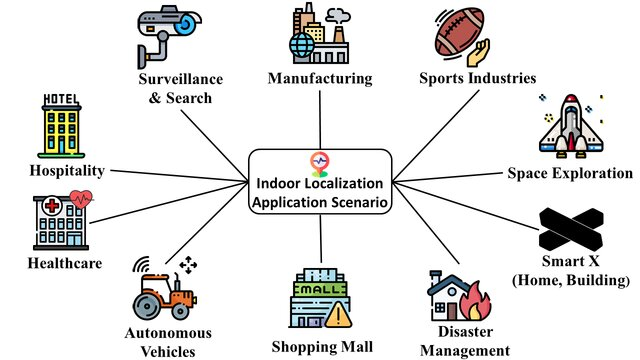
\includegraphics[width=0.75\linewidth]{../FloorLocalization/images/Applications.jpg}
		\caption{Applications \cite{Caltagirone:2021}}
	\end{figure}
	\pagebreak
	\textbf{Industrial and Commercial}
	\begin{itemize}
		\item Warehouse automation and inventory management. \cite{Singh:2023}
		\item Manufacturing robot navigation and coordination. \cite{Camacho-Escobar:2020}
		\item Retail customer analytics and indoor directions. \cite{Singh:2023}
	\end{itemize}
	\textbf{Smart Buildings and IoT}
	\begin{itemize}
		\item Building management and space utilization.\cite{Wang:2024}
		\item Asset tracking and security monitoring.\cite{Wang:2024}
		\item Environmental sensing and control systems.\cite{Luo:2020}
	\end{itemize}
}

\Mysection{Algorithm}

\STANDARD{Flowchart for Mobile Robot Navigation}
{
	\begin{figure}
		\centering 
		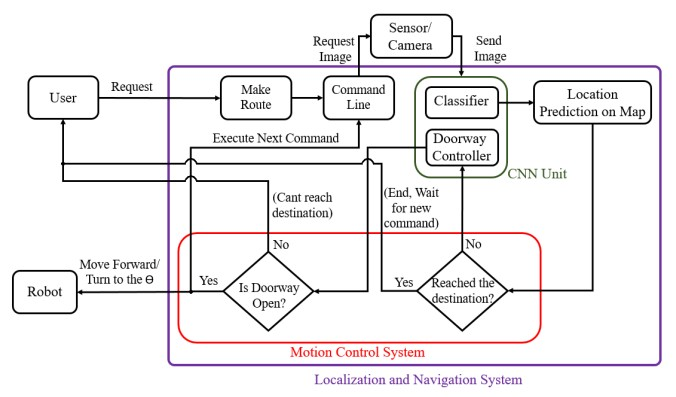
\includegraphics[width=0.9\linewidth]{../FloorLocalization/images/flowchartnavigation.jpg}
		\caption{Flowchart for Mobile Robot Navigation\cite{Foroughi:2021}}
	\end{figure}
}
\STANDARD{Flowchart for Indoor Localization}
{
 	\begin{figure}
 		\centering 
 		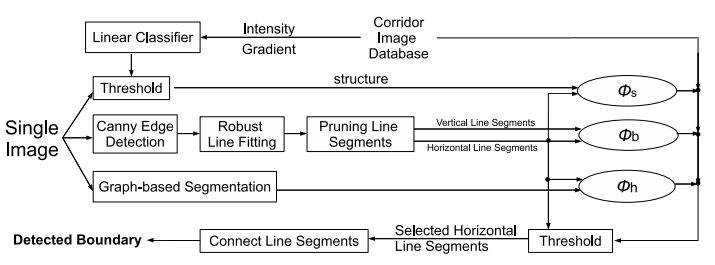
\includegraphics[width=\linewidth]{../FloorLocalization/images/Flowchart.png}
 		\caption{Flowchart for floor detection\cite{Li:2010}}
 	\end{figure}
}
\STANDARD{Mathematical Expression}
{
	To determine the likelihood that a horizontal segment $\ell_h$ is near this boundary, we compute a weighted sum of scores for three individual visual cues:
	\begin{equation}
		\Phi_{total}(\ell_h) = w_s \overline{\phi}_s(\ell_h) + w_b \overline{\phi}_b(\ell_h) + w_h \overline{\phi}_h(\ell_h),
	\end{equation}
	where $w_s, w_b,$ and $w_h$ are the weights, and $\overline{\phi}_s(\ell_h), \overline{\phi}_b(\ell_h), \overline{\phi}_h(\ell_h)$ are the three individual scores, which are now described.\cite{Li:2010}
}

\Mysection{Hardware Platform: Jetson Nano and Raspberry Pi Camera}

\STANDARD{Nvidia Jetson Nano}
{
\textbf{System Architecture}

    The NVIDIA Jetson Nano developer kit paired with Raspberry Pi Camera Module provides an optimal platform for embedded computer vision applications
	\begin{figure}
		\centering
		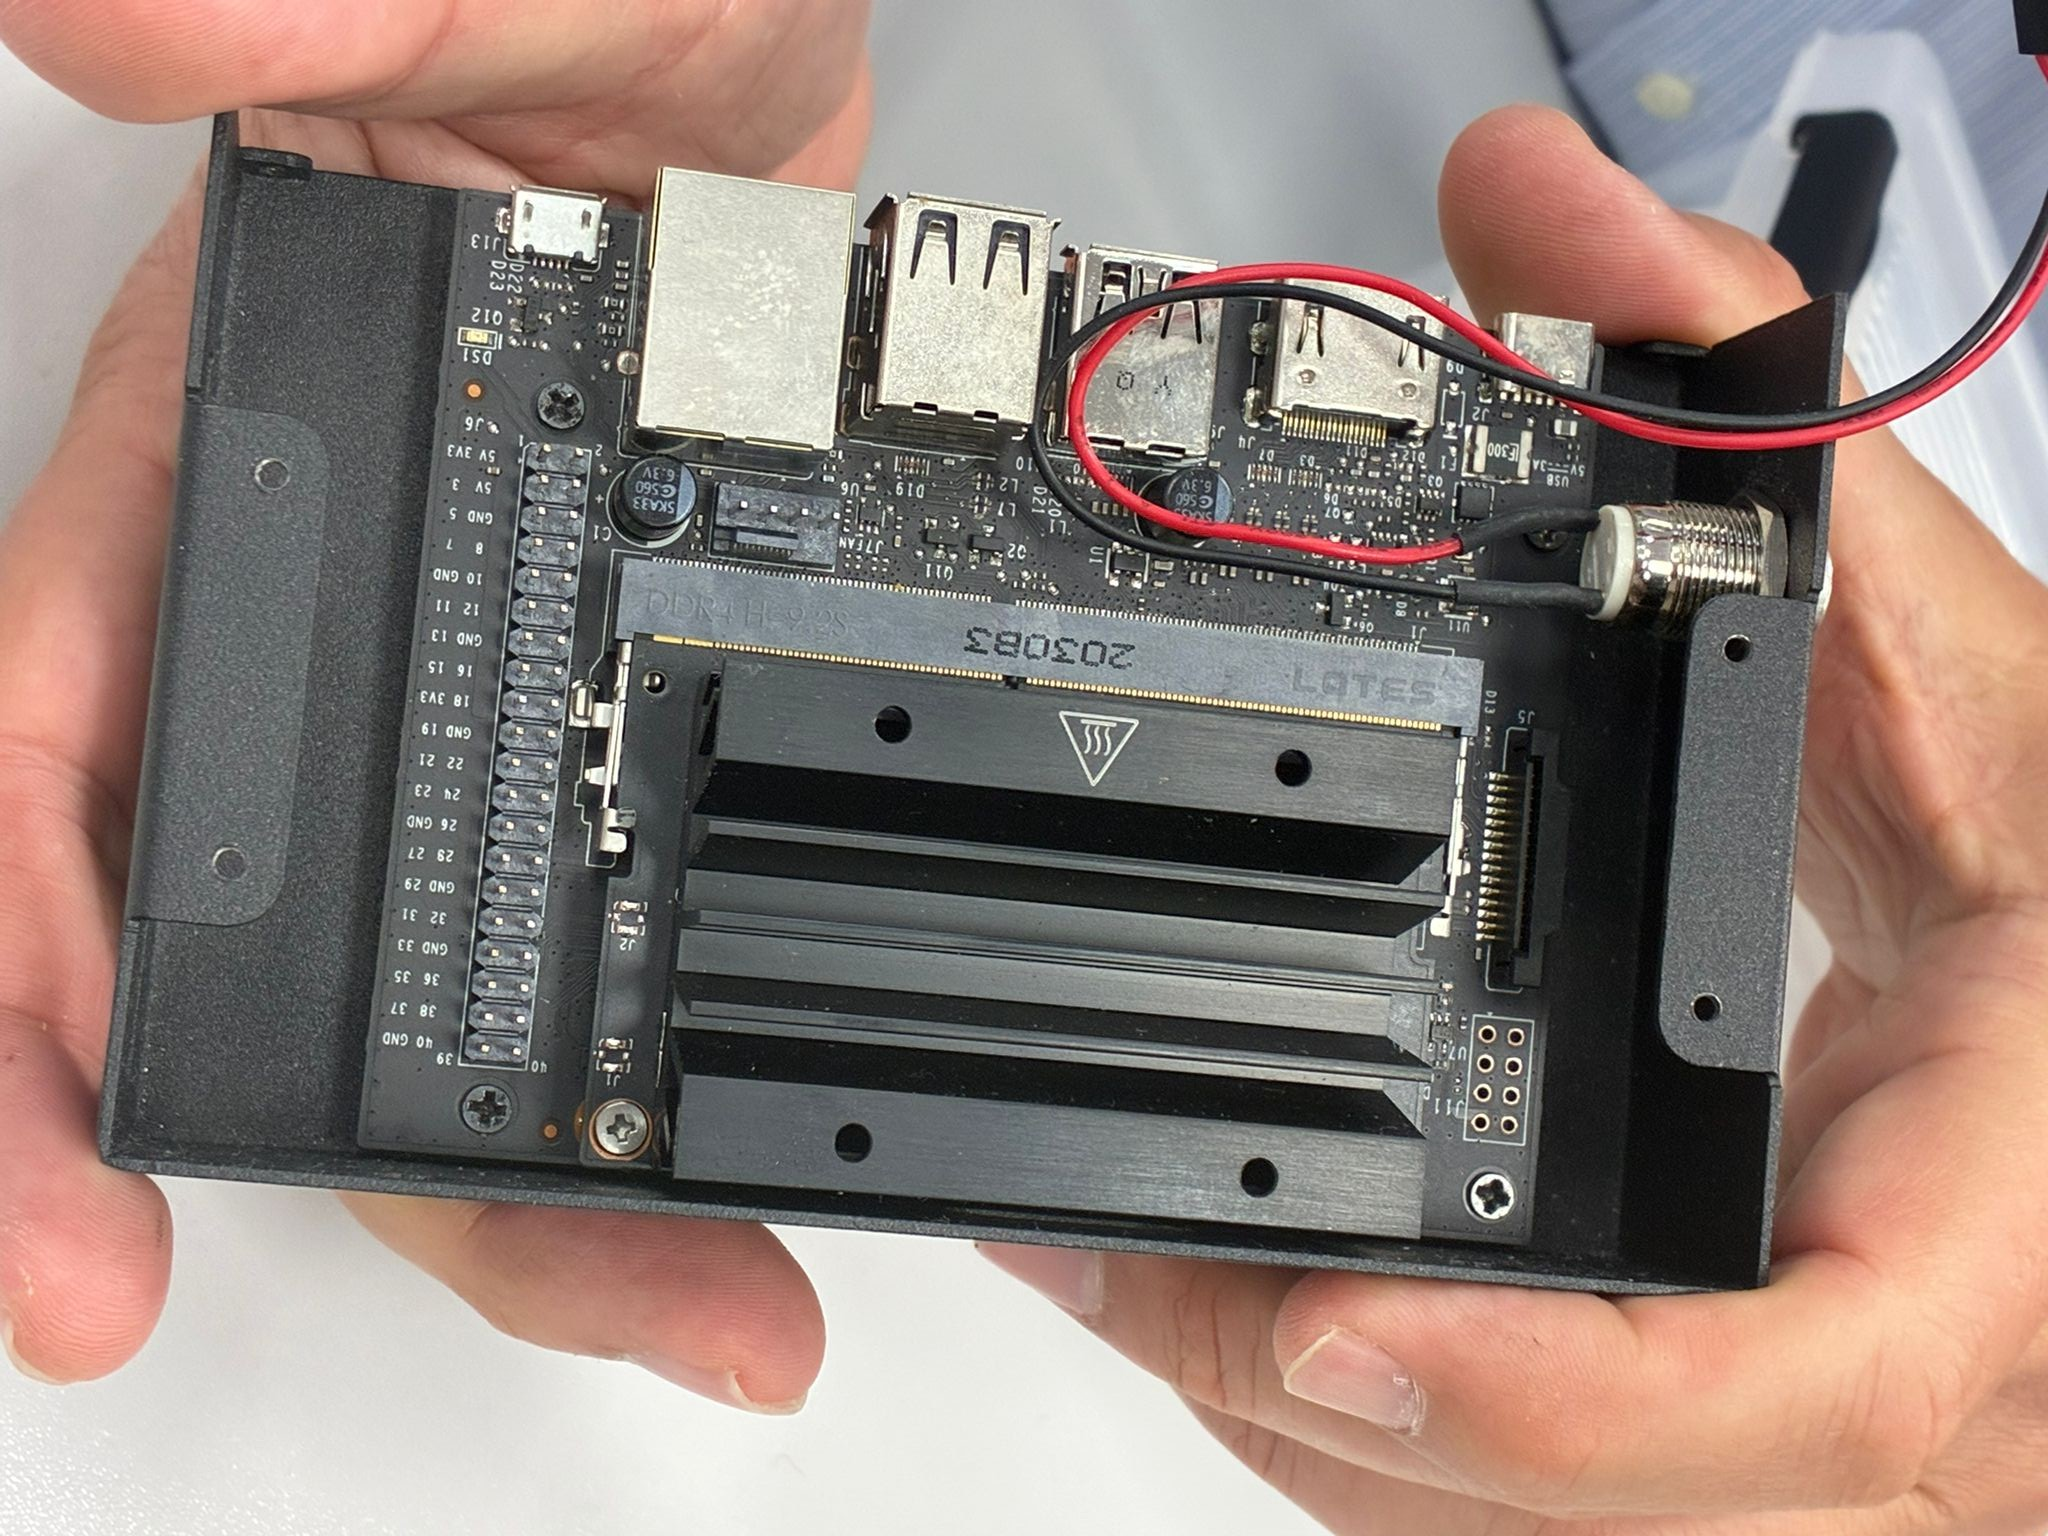
\includegraphics[width=0.4\linewidth]{../FloorLocalization/images/JetsonNano.jpeg}
		\caption{Nvidia Jetson Nano}
	\end{figure}
	\pagebreak
	\begin{figure}
		\centering
		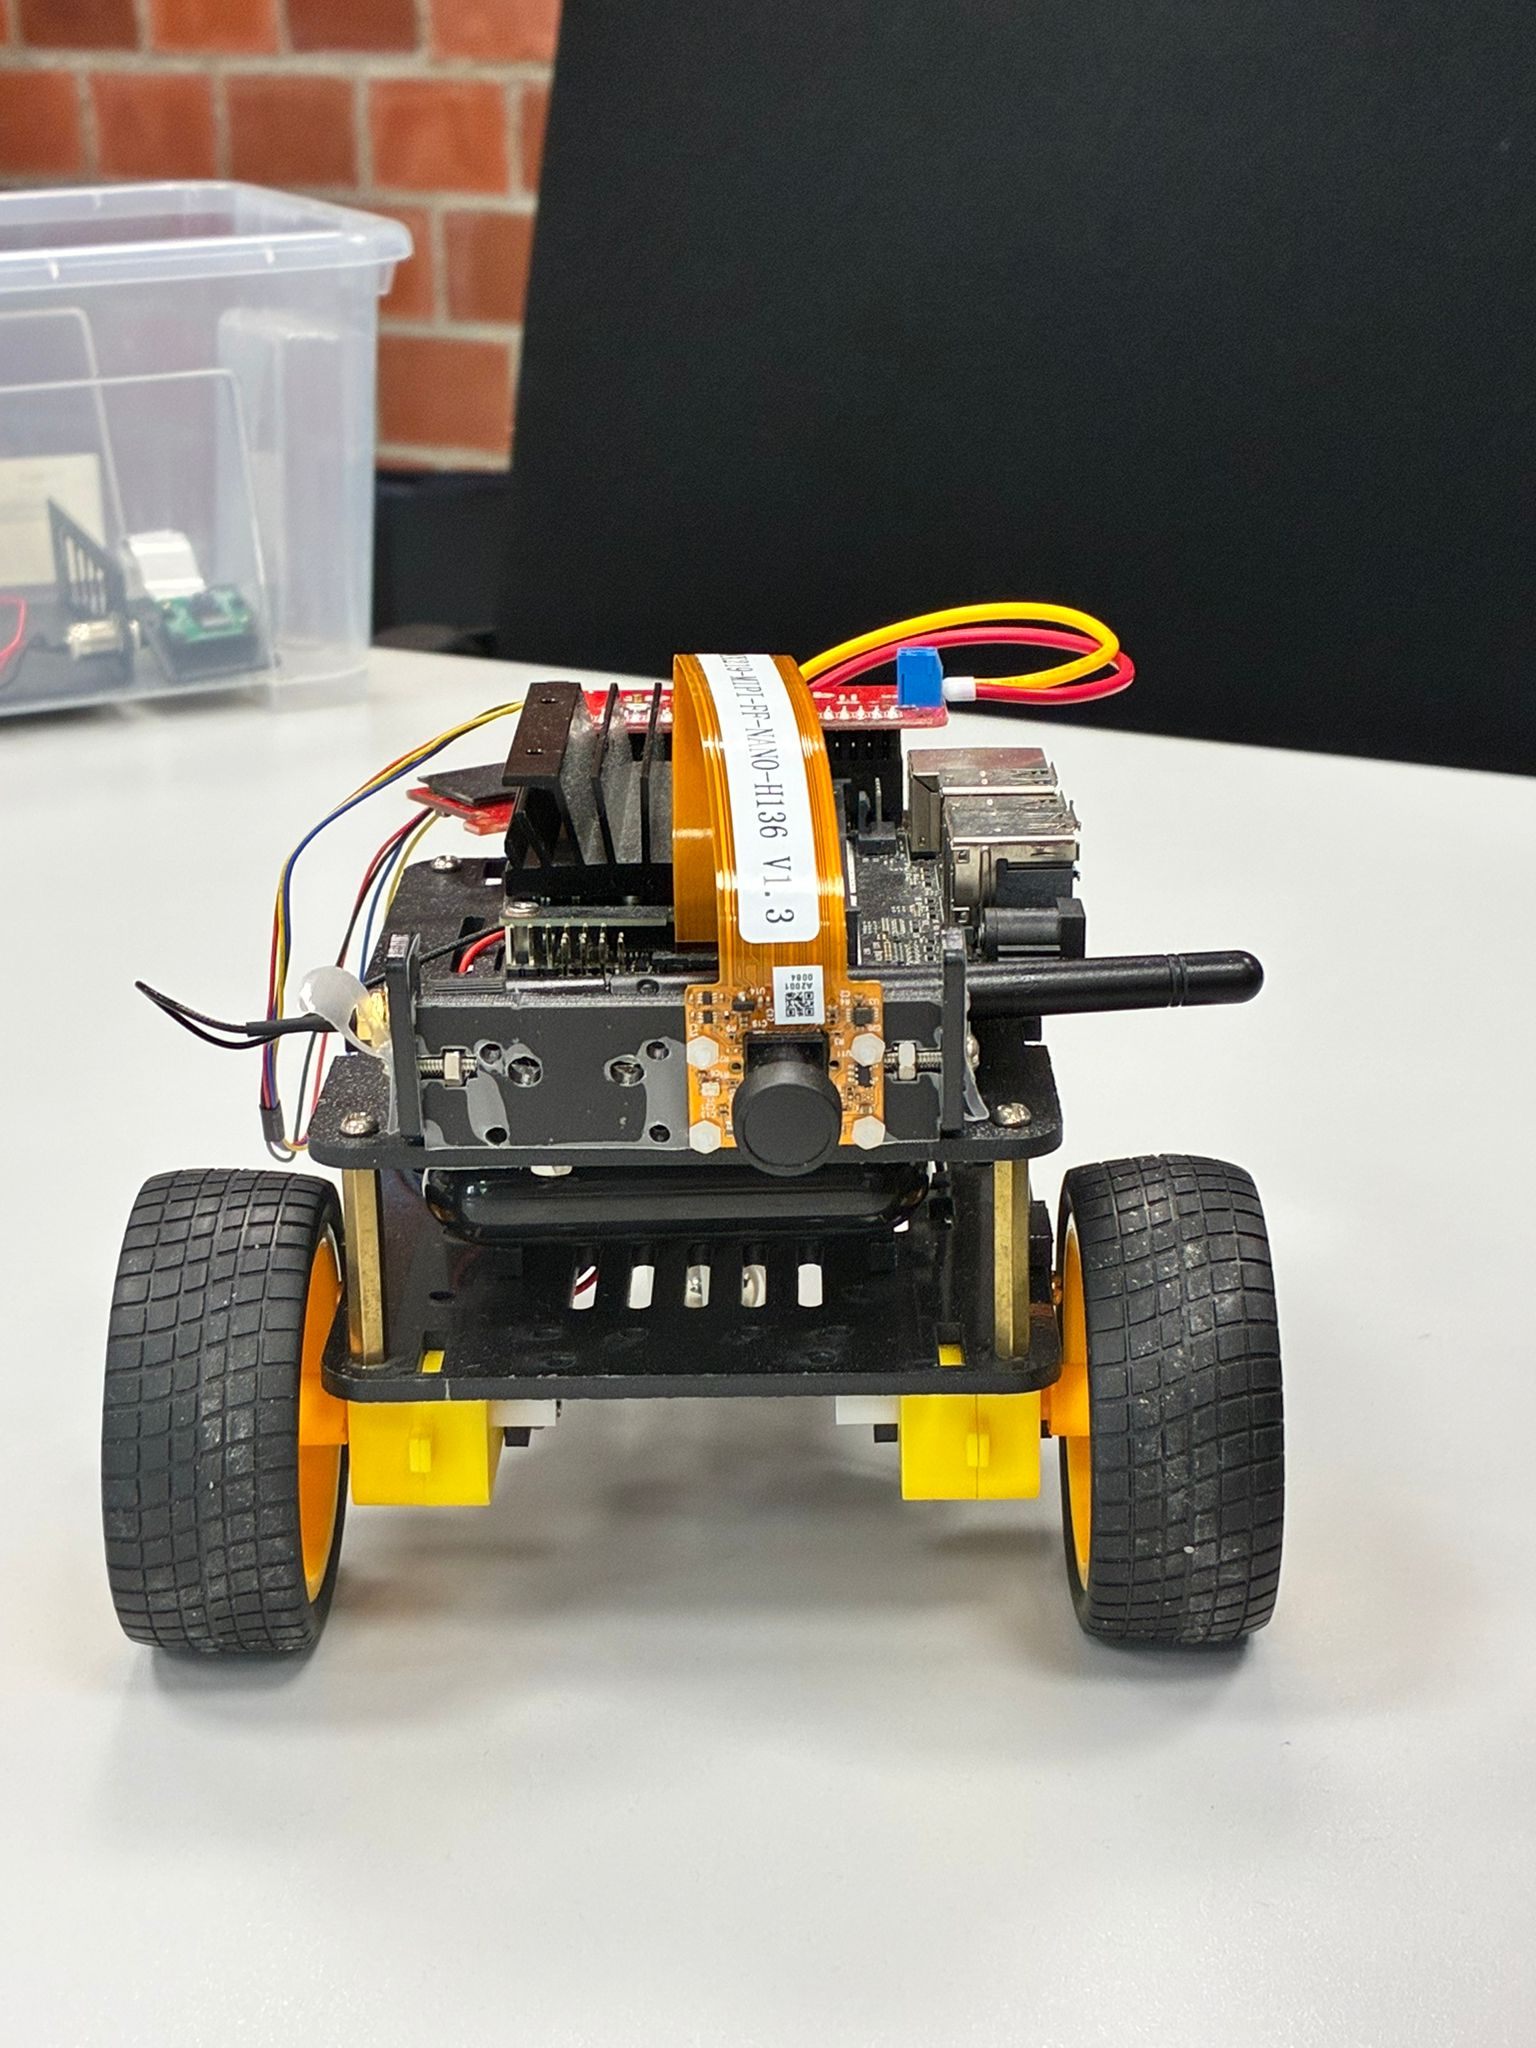
\includegraphics[width=0.4\linewidth]{../FloorLocalization/images/RaspberryPiCam.jpeg}
		\caption{Mobile Robot with Raspberry Pi camera (Front view)}
	\end{figure}
	\pagebreak
    Hardware Specifications
    \begin{itemize}
        \item \textbf{Jetson Nano}: ARM Cortex-A57 quad-core processor, 128-core Maxwell GPU
	    \item \textbf{Camera}: Raspberry Pi Camera Module V2 (8MP, 1080p, Sony IMX219 sensor)
	    \item \textbf{Interface}: 15-pin MIPI CSI-2 connection for direct camera integration
		\item \textbf{Processing}: Hardware-accelerated computer vision with CUDA support
    \end{itemize}
	
}
\Mysection{KDD implementation in Floor Localization} 
\STANDARD{Machine Learning Pipeline}
{
	\begin{figure}
		\centering
		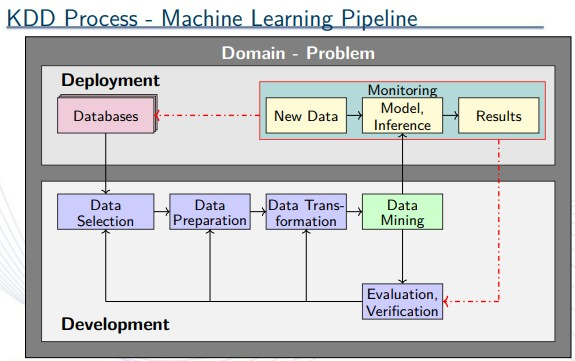
\includegraphics[width=0.8\linewidth]{../FloorLocalization/images/KDD.jpg}
		\caption{KDD Process - ML Pipeline}
	\end{figure}
}
\STANDARD{KDD Implementation for Floor Localization}{
	\begin{itemize}
		\item Problem understanding: robust indoor floor localization for a mobile robot to support safe navigation and obstacle avoidance; real-time inference on embedded hardware (Jetson Nano) from a Raspberry Pi Camera stream under edge-compute constraints \cite{Luo:2020,Camacho-Escobar:2020}.
		\item Data understanding and database: sources are RGB frames (CSI-2), optional IMU (accelerometer/gyroscope), environment metadata (lighting, floor material), and ground truth via annotated floor boundaries and pose labels \((x,y,\theta)\); streams feature high velocity, varied textures, and illumination changes \cite{Foroughi:2021,Zhang:2019}.
		\pagebreak
		\item Data selection: retain frames with adequate texture/edges, acceptable shutter time, low blur; select edge maps, line segments, vanishing-point cues, optical flow, and IMU channels for fusion \cite{SP-VIO:2024,Trifo-VIO:2018}.
		\item Data preparation: calibrate/undistort camera, normalize exposure and white balance, deblur/denoise; time-synchronize camera and IMU, remove outliers, interpolate short dropouts; split by location/session to prevent leakage \cite{RMSC-VIO:2024,VIO-DualProNet:2024}.
		\pagebreak
		\item Data transformation: engineer features (Canny, line detection, graph/superpixel cues, optical-flow summaries), normalize image/IMU signals and pose units, augment with brightness/contrast jitter, rotations, crops, perspective warps \cite{SG-VIO:2024,360-VIO:2024,RD-VIO:2024}.
		\item Data mining (modeling): use a lightweight CNN for floor/non-floor and boundary likelihoods optimized with TensorRT on Jetson Nano; fuse CNN measurements with IMU via EKF/VIO for drift reduction; output \((x,y,\theta)\) and uncertainty, optionally updating a floor/occupancy map \cite{Load-Balanced-SBA:2024,PLI-VIO:2023,PGD-VIO:2024}.
		\pagebreak
		\item Evaluation and verification: report ATE/RPE, boundary IoU/F1, route success rate, and on-device latency/FPS; validate with k-fold across rooms/floors, stress tests (illumination/occlusions), and ablations (vision-only vs.\ vision+IMU) \cite{Latency-Compensated-VIO:2020,Point-Line-VIO:2024}.
		\item Deployment: export to ONNX and TensorRT with fixed input (e.g., \(256\times256\)), integrate pose/uncertainty into the motion controller to issue velocity/turn commands with safety stops \cite{EMA-VIO:2022,PIEKF-VIWO:2023}.
		\item Monitoring and maintenance: track pose error vs.\ landmarks, FPS, dropped frames, IMU bias; detect data drift, log failures for replay, periodically fine-tune and re-check calibration.
	\end{itemize}
}

